%%%%%%%%%%%%%%%%%%%%%%%%%%%%%%%%%%%%%%%%%
% Journal Article
% LaTeX Template

\documentclass{article}

\usepackage{hyperref}
\usepackage[sc]{mathpazo} % Use the Palatino font
\usepackage[T1]{fontenc} % Use 8-bit encoding that has 256 glyphs
\linespread{1.3} % Line spacing - Palatino needs more space between lines
\usepackage{microtype} % Slightly tweak font spacing for aesthetics
\usepackage{listings}             % Include the listings-package
\usepackage[hmarginratio=1:1,top=32mm,columnsep=20pt]{geometry} % Document margins
\usepackage{multicol} % Used for the two-column layout of the document
\usepackage[hang, small,labelfont=bf,up,textfont=it,up]{caption} % Custom captions under/above floats in tables or figures
\usepackage{booktabs} % Horizontal rules in tables
\usepackage{float} % Required for tables and figures in the multi-column environment - they need to be placed in specific locations with the [H] (e.g. \begin{table}[H])
\usepackage{hyperref} % For hyperlinks in the PDF
\usepackage{graphicx}
\usepackage{pdfpages}
\graphicspath{.}
\usepackage{abstract} % Allows abstract customization
\renewcommand{\abstractnamefont}{\normalfont\bfseries} % Set the "Abstract" text to bold
\renewcommand{\abstracttextfont}{\normalfont\small\itshape} % Set the abstract itself to small italic text

\usepackage{titlesec} % Allows customization of titles
\renewcommand\thesection{\Roman{section}} % Roman numerals for the sections
\renewcommand\thesubsection{\Roman{subsection}} % Roman numerals for subsections

\usepackage{fancyhdr} % Headers and footers
\pagestyle{fancy} % All pages have headers and footers
\fancyhead{} % Blank out the default header
\fancyfoot{} % Blank out the default footer
\fancyhead[C]{BINP25 project $\bullet$ October 2016 } % Custom header text
\fancyfoot[RO,LE]{\thepage} % Custom footer text

%----------------------------------------------------------------------------------------
%	TITLE SECTION
%----------------------------------------------------------------------------------------

\title{\vspace{1mm}\fontsize{16pt}{12pt}\selectfont\textbf{Analysis of tri-axial accelerometer data of 4 month old infants}} % Article title

\author{
\large
\text{Student:}
\textsc{Jerneja Mislej}\\[2mm] % Your name
\normalsize University of Lund \\ % Your institution
\normalsize \href{mailto:bif15jmi@student.lu.se}{bif15jmi@student.lu.se}\\\\ % Your email address
\large
\text{Project supervisor:}
\textsc{Frida Renstrom}\\[2mm] % Your name
\normalsize University of Lund \\ % Your institution
\normalsize \href{mailto:Frida.Renstrom@med.lu.se}{Frida.Renstrom@med.lu.se}\\ % Your email address
\large \\
\text{Assistant project supervisors:}
\textsc{Paul W. Franks, Azra Kurbasic}\\[2mm] % Your name
\normalsize University of Lund \\ % Your institution
\normalsize \href{mailto:Paul.Franks@med.lu.se}{Paul.Franks@med.lu.se}\\ \\% Your email address
\normalsize \href{mailto:Azra.Kurbasic@med.lu.se}{Azra.Kurbasic@med.lu.se}\\
\vspace{-5mm}
}
\date{}


%----------------------------------------------------------------------------------------

\begin{document}

\maketitle % Insert title

\thispagestyle{fancy} % All pages have headers and footers

%---------------------------------ph-------------------------------------------------------
%	ABSTRACT
%----------------------------------------------------------------------------------------

\begin{abstract}

\noindent 
\fontsize{10pt}{11pt}\selectfont {The main goal of the project is to extract physical activity levels from tri-axial accelerometer data, taken of 4 month old infants. Infants wore two accelerometers, one on the torso, other on the ankle, for 48 hours in a free living environment. In order to properly extract physical activity, the accelerometer data has to be prepared and preprocessed. Preparation includes data organization and timestamp alignment, while the preprocessing includes filtering, averaging, removal of data where the accelerometer was not worn, summary measure extraction, correction for gravity component and correction for acceleration contributed by the infants caretaker. Several approaches are discussed and presented along with the problems and negative features of each. The results from the correction of accelerations due to infant being moved are compared against the diary notations of infants sleeping and feeding habits, kept by their mothers. In the end, physical activity levels are extracted and analyzed along with other variables.
\\\\}

\end{abstract}

%----------------------------------------------------------------------------------------
%	ARTICLE CONTENTS
%----------------------------------------------------------------------------------------



\newpage
\begin{narrow}
\begin{table}[h]
\begin{tabular}{|p{1.2cm}|p{2cm}|p{2cm}|p{2cm}|p{2cm}|p{2cm}|p{2cm}|}
\hline
over all &\multicolumn{2}{c|}{mean of summary} &\multicolumn{2}{c|}{mean SD of being moved blocks} & \multicolumn{2}{c|}{\parbox[c]{4cm}{variation of SD of being\\moved blocks}}\\ \cline{2-7} 
         & torso & ankle & torso & ankle & torso & ankle \\ \hline
mean     & -2.362e-13 g & 2.099e-12 g & 0.0065 g & 0.0131 g & 0.0045 g & 0.0065 g \\ \hline
sd       & 0.0061 g & 0.0112 g & 0.0011 g & 0.0020 g & 0.0010 g & 0.0023 g \\ \hline
min      & -0.3132 g & -0.3134 g & 0.0044 g & 0.0103 g & 0.0033 g & 0.0040 g \\ \hline
max      & 0.3348 g & 0.3551 g & 0.0092 g & 0.0183 g & 0.0072 g & 0.0148 g \\ \hline
\end{tabular}
\end{table}
\end{narrow}
\\

newline\\
\\
\\
\\
average torso min of SD = 0.0013g\\
average torso max of SD = 0.0237g\\
average ankle min of SD = 0.0021g\\
average ankle max of SD = 0.0338g\\
%----------------------------------------------------------------------------------------
%	REFERENCE LIST
%----------------------------------------------------------------------------------------
\newpage
\begin{thebibliography}{99} 
\end{thebibliography}
%----------------------------------------------------------------------------------------
\\
\\
\\
\\
\\
\\
\\
\\
\\
\Large{\textbf{Supplements}}
\\
\\
\normalsize Example of a diary kept by the infants mother.
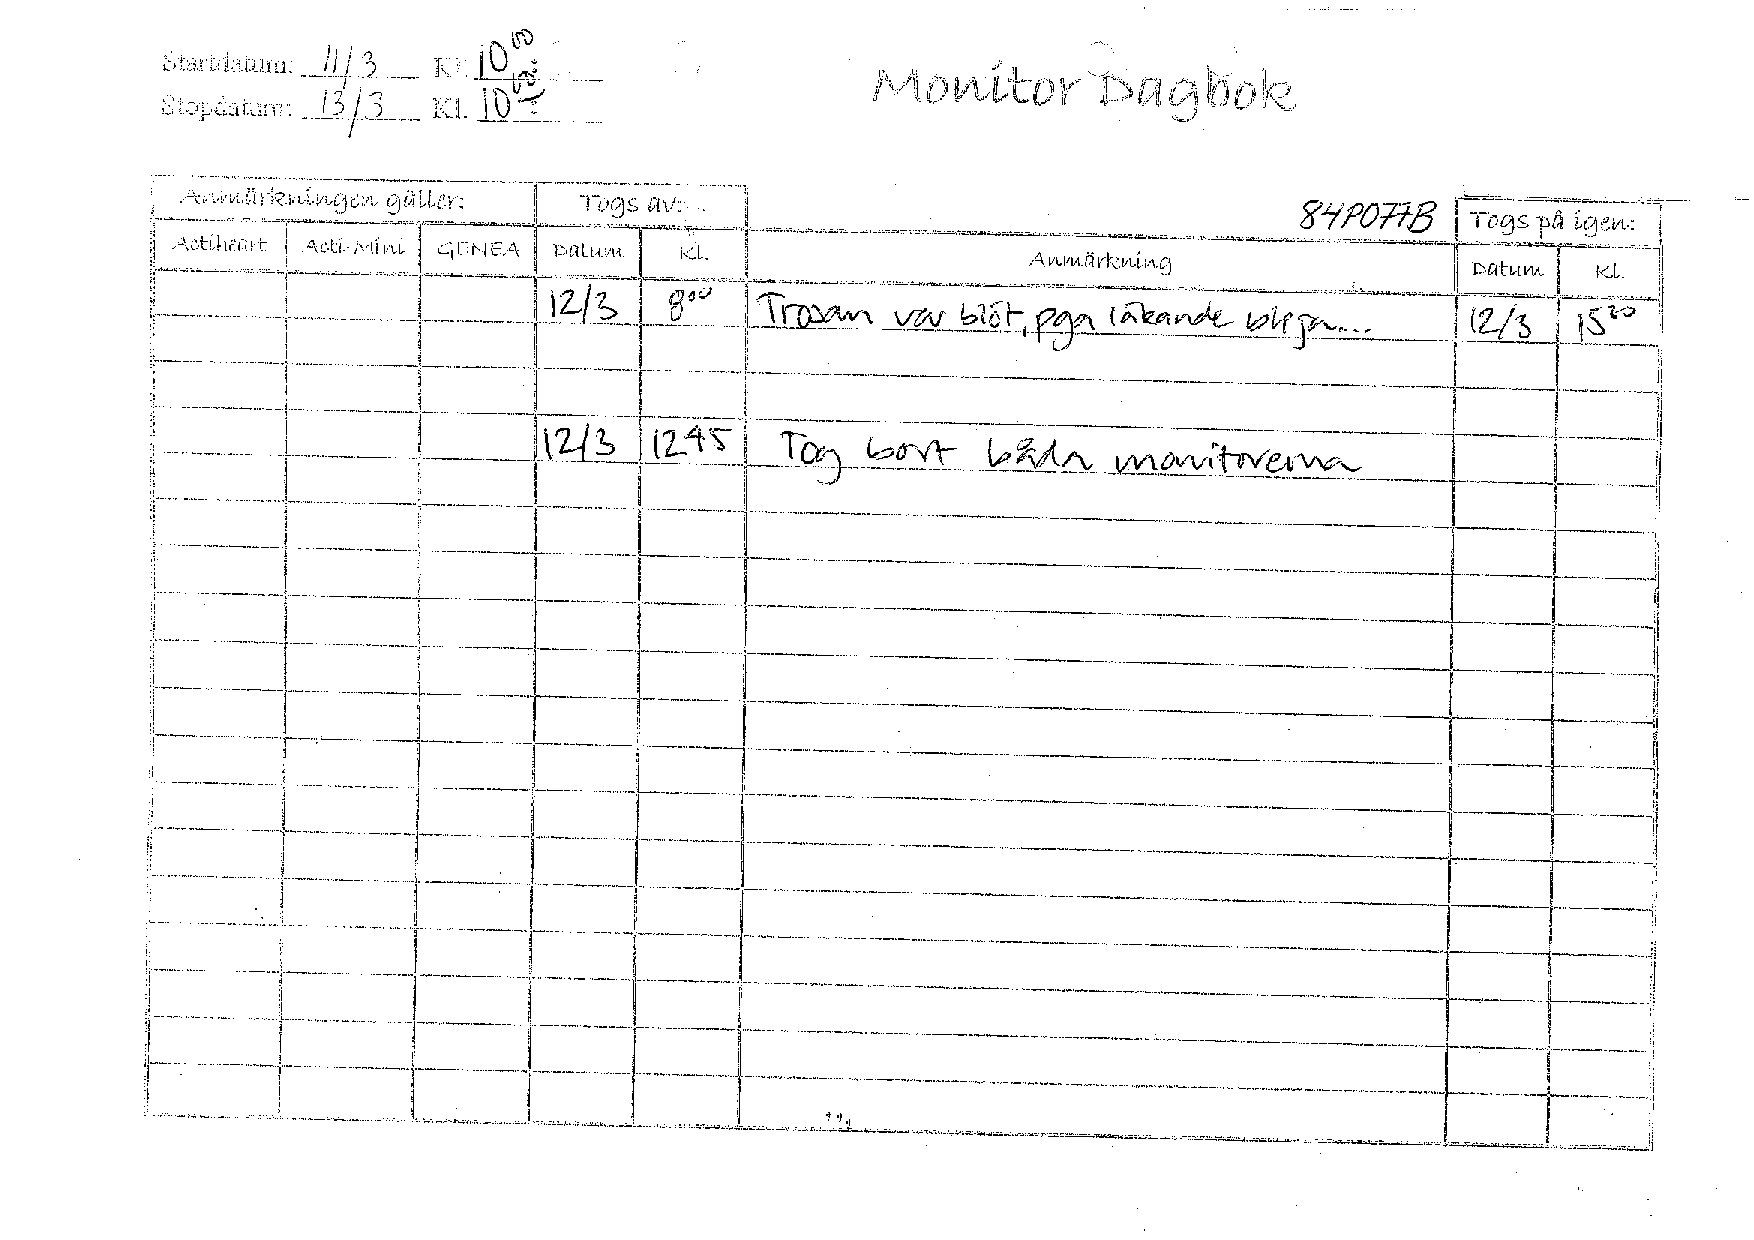
\includepdf[pages=-]{friendly_84P077.pdf}
\end{document}based
